\section{A compressed graph representation of arc consistency}
\label{comp:section}

Throughout this section, $r\geq 3$, $K=r+1$, and all vector spaces and
affine maps are over $\F_2$.  The construction stores only two consecutive
coordinates of an address in each block.  A complete address becomes
visible to the game through a ring of $r$ blocks.  A close structural
parallel appears in the compressed CFI construction of Grohe, Lichter,
Neuen, and Schweitzer: row periods involving neighboring moduli compress
a product-length cylindrical grid.  In the periodic lift, their separator
lemmas show, under their stated hypotheses, that changing one row
representative changes the unique separator meeting every row once in at
most one vertex
\cite[Section~5, Lemmas~19, 29, and~30]{CFICompression}.  The scalar-image
consistency and exact offset-extension properties used here are proved below.

\subsection{The consistency instance}

Put $[m]=\{0,\ldots,m-1\}$, where $m\geq 2$.  Fix a finite collection
$\mathcal P$ of \emph{real types}, with a dimension $d_P$ for each
$P\in\mathcal P$.  The variables
of type $P$ are indexed by $\mathbf a\in[m]^r$ and take values in
$\F_2^{d_P}$.  An \emph{edge schema} $e$ specifies ordered endpoint types
$P,R$, possibly equal, together with the following data:
\begin{itemize}
\item For each coordinate $i$, a set $A_{e,i}\subseteq[m]$ and an injection
  $\sigma_{e,i}\colon A_{e,i}\longrightarrow[m]$.
\item An affine form $\phi_{e,0}(u)=\lambda_{e,0}u+d_{e,0}$ at $P$ and
  an affine form $\phi_{e,1}(u)=\lambda_{e,1}u+d_{e,1}$ at $R$.
\end{itemize}
The forms are scalar valued; their linear parts may be zero.  Write
$A_e=\prod_i A_{e,i}$ and
$\boldsymbol\sigma_e(\mathbf a)=(\sigma_{e,i}(a_i))_{i=1}^r$.
For every $\mathbf a\in A_e$, the schema gives one individual comparison
between $\phi_{e,0}$ at $(P,\mathbf a)$ and $\phi_{e,1}$ at
$(R,\boldsymbol\sigma_e(\mathbf a))$.

\begin{definition}\label{comp:ac}
The instance has \emph{individual-edge arc consistency} if there are
nonempty sets $Q_{P,\mathbf a}\subseteq\F_2^{d_P}$, for every real type
and every address, such that
\begin{equation}\label{comp:ac-equation}
 \phi_{e,0}(Q_{P,\mathbf a})
 =\phi_{e,1}(Q_{R,\boldsymbol\sigma_e(\mathbf a)})
 \qquad(e,\ \mathbf a\in A_e).
\end{equation}
Each equality is imposed separately.  In particular, parallel comparisons
are not combined into a single relation.
\end{definition}

This is a per-comparison local-support condition, in the tradition of arc
consistency \cite[Section~4]{Mackworth1977}. Every possible value at one
endpoint must have a supporting value at the other, but the support may
depend on the value and on the comparison. Even when a schema has the
same type and address at both ends, its two endpoint occurrences may
use different vectors from the same set. We do not ask for one globally
compatible vector at every address.

A \emph{description shape} fixes the types, their dimensions, and the
number and incidence of the schemas.  The coordinate sets and maps can
depend on $m$.  They are specified by their one-coordinate tables.
The scalar forms may vary as well, but their descriptions have bounded
size because the dimensions and number of schemas are fixed.

\begin{theorem}[Compressed consistency reduction]\label{comp:reduction}
For fixed $r$ and fixed description shape, an instance as above determines
two equally large simple uncolored connected graphs $G^0,G^1$, of
diameter at most two and order
\[
                         O_{r,\mathrm{shape}}(m^6),
\]
such that Duplicator wins the $K$-pair bijective game on $G^0,G^1$ if and
only if the instance has individual-edge arc consistency.
The construction uses the bounded scalar-form data together with the
one-coordinate tables, and enumerates $O_{r,\mathrm{shape}}(m^2)$ blocks
without enumerating all full addresses.
An arbitrary equal number of additional vertices can be added to the two
graphs while preserving the equivalence, connectedness, and diameter
bound.
\end{theorem}

We prove the theorem in several steps.  An unused real type of dimension
one may be added at the outset.  This does not affect consistency and
ensures that the constructions below have at least two valuation vertices.

\subsection{Subdivided types and local blocks}

Replace each schema by a path with $4(r+1)$ private internal types, each
of dimension one.  Call this subdivided path a \emph{wire}; its endpoints
are the original real types, and its segments are \emph{links}.
At an internal type of schema $e$,
the allowed labels in coordinate $i$ are $A_{e,i}$; at a real type all
labels in $[m]$ are allowed.  Along the path the coordinate matches are
identity matches on these allowed labels, except at the second real
endpoint, where the match is $p\mapsto\sigma_{e,i}(p)$.

For a link $\ell$ with endpoints $t,u$, its scalar comparison has the form
\begin{equation}\label{comp:link}
                         L_{\ell,t}h_t+L_{\ell,u}h_u=b_\ell.
\end{equation}
The notation for a linear form is local to its link and endpoint.  An
internal link has both forms equal to the identity and $b_\ell=0$.
At a real endpoint use the linear part of its original affine form,
identity at the internal endpoint, and the constant term as $b_\ell$.
Thus the internal scalar carries the value of the original affine form.
For use only in the analysis, extend each coordinate injection to a
permutation of $[m]$; the actual links retain only their allowed matches.

Boundary indices $i=1,\ldots,r$ are cyclic, with $r+1$ denoting boundary
$1$.  Put $\delta_i=1$ for $i=r$ and $\delta_i=0$ otherwise.  A
\emph{corner} is a triple $(i,t,p)$, where $p$ is an allowed label at
boundary $i$ of type $t$.  We use two kinds of blocks.
\begin{itemize}
\item A \emph{site block} at type $t$, row $i$, and allowed labels $p,p'$
  has one vector readout $x\in\F_2^{d_t}$.  Its name is the horizontal
  edge from $(i,t,p)$ to $(i+1,t,p')$.  All values are allowed.
\item A \emph{square block} at link $\ell=tu$, row $i$, and allowed
  matches at boundaries $i,i+1$ has the two corresponding horizontal
  readouts $x_t,x_u$ and two scalar vertical readouts $y_i,y_{i+1}$.
  A vertical readout is named by its boundary, link, and label match.
  In version $\varepsilon\in\{0,1\}$ the permitted valuations satisfy
  \begin{equation}\label{comp:square}
   L_{\ell,t}x_t+L_{\ell,u}x_u+y_i+y_{i+1}
                           =\varepsilon\delta_i b_\ell.
  \end{equation}
\end{itemize}
Version $0$ is called homogeneous and version $1$ affine.  Two occurrences
of a readout with the same name denote the same vector or scalar.  A
\emph{valuation} of a block specifies all its readouts.  The legal
valuations of any block form a linear space in version $0$ and a
nonempty affine coset of that space in version $1$.  For a square this
follows, for example, from the coefficient one of $y_i$ in
\eqref{comp:square}.

For the moment, construct vertex-colored graphs: the vertices are legal
block valuations, and each block has its own color.  Between two distinct
blocks sharing at least one readout name, place an edge exactly when
the valuations agree on \emph{all} their shared readouts.  There are no
other edges.  Corresponding blocks have equally many vertices in the
two graphs.

\begin{figure}[htbp]
\centering
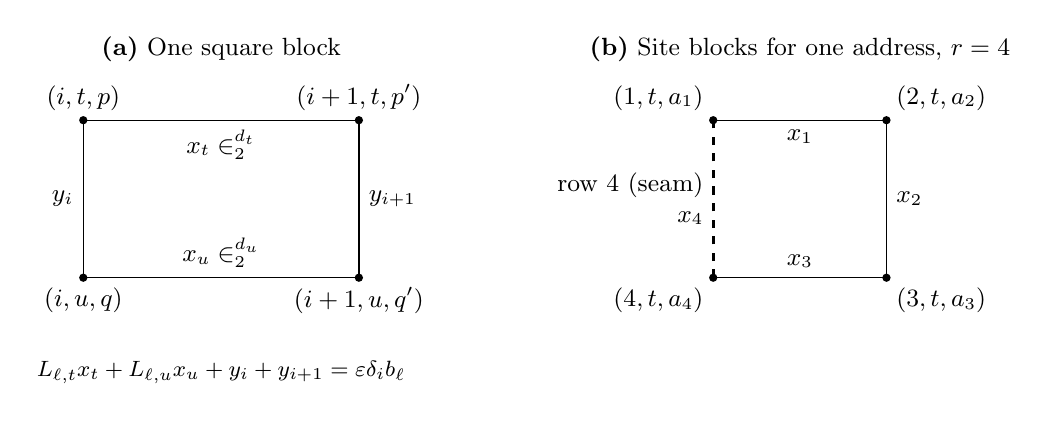
\begin{tikzpicture}[font=\small,line width=0.5pt]
  \node at (1.75,0.9) {\textbf{(a)} One square block};
  \draw (0,0) -- (3.5,0) -- (3.5,-2) -- (0,-2) -- cycle;
  \fill (0,0) circle (1.5pt);
  \fill (3.5,0) circle (1.5pt);
  \fill (3.5,-2) circle (1.5pt);
  \fill (0,-2) circle (1.5pt);
  \node[above] at (0,0) {$(i,t,p)$};
  \node[above] at (3.5,0) {$(i+1,t,p')$};
  \node[below] at (0,-2) {$(i,u,q)$};
  \node[below] at (3.5,-2) {$(i+1,u,q')$};
  \node[below] at (1.75,0) {$x_t\in\F_2^{d_t}$};
  \node[above] at (1.75,-2) {$x_u\in\F_2^{d_u}$};
  \node[left] at (0,-1) {$y_i$};
  \node[right] at (3.5,-1) {$y_{i+1}$};
  \node[font=\footnotesize] at (1.75,-3.2)
    {$L_{\ell,t}x_t+L_{\ell,u}x_u+y_i+y_{i+1}
       =\varepsilon\delta_i b_\ell$};

  \node at (9.1,0.9) {\textbf{(b)} Site blocks for one address, $r=4$};
  \draw (8,0) -- (10.2,0) -- (10.2,-2) -- (8,-2);
  \draw[dashed,very thick] (8,-2) -- (8,0);
  \fill (8,0) circle (1.5pt);
  \fill (10.2,0) circle (1.5pt);
  \fill (10.2,-2) circle (1.5pt);
  \fill (8,-2) circle (1.5pt);
  \node[above left] at (8,0) {$(1,t,a_1)$};
  \node[above right] at (10.2,0) {$(2,t,a_2)$};
  \node[below right] at (10.2,-2) {$(3,t,a_3)$};
  \node[below left] at (8,-2) {$(4,t,a_4)$};
  \node[below] at (9.1,0) {$x_1$};
  \node[right] at (10.2,-1) {$x_2$};
  \node[above] at (9.1,-2) {$x_3$};
  \node[left,align=right] at (8,-1) {row $4$ (seam)\\$x_4$};
\end{tikzpicture}
\caption{Corner and readout geometry.  Dots are corners; each vertex
of a valuation graph is a legal valuation of an entire block.
In (a), horizontal edges name vector readouts and vertical edges name
scalar readouts for the two allowed label matches.  Each horizontal
edge also specifies its corresponding site block.
In (b), a fixed type and allowed address $(a_1,a_2,a_3,a_4)$ select
four separate site blocks, with row $4$ crossing the cyclic seam.
All four edges in (b) name site readouts.  Blocks share a readout
through a common named edge; meeting only at a corner does not suffice.}
\label{comp:readout-figure}
\end{figure}

\subsection{Reading a comparison}

\begin{lemma}\label{comp:necessity}
A block-preserving winning strategy with $r+1$ pairs implies
individual-edge arc consistency.
\end{lemma}
\begin{proof}
Spoiler always selects zero valuations in the homogeneous graph.  They
are legal in every block.  Whenever two pebbled distinct blocks share
readouts, their selected zero valuations are adjacent, so their answers
must agree on every shared readout.

We may regard a finite query as ending immediately after discards, by
the removal closure of winning positions from Section~\ref{game:section}.

Fix a type $t$ and an allowed full address.  Its \emph{site ring} consists
of the $r$ site blocks using the address labels at consecutive boundaries,
as illustrated in Figure~\ref{comp:readout-figure}(b).
The sum of their answered horizontal readouts is a value
$h_t\in\F_2^{d_t}$.  To cross a link at a matched address, replace these
site blocks by their corresponding square blocks, one row at a time:
place the square while retaining its old site, and then discard the
site.  This uses at most $r+1$ pairs and preserves each old horizontal
readout on the $t$ side.  When all $r$ squares are pebbled, their vertical
readouts agree at adjacent boundaries.  Summing \eqref{comp:square} in
the affine graph gives \eqref{comp:link} for the sums on the two sides.
Now replace the squares, in the same manner, by the site ring at $u$.
Its sum is preserved from the $u$ side of the squares.  Repeating along
the subdivided path transmits the original affine comparison.  The same
procedure works in reverse.

Fix a winning strategy.  Let $Q_{P,\mathbf a}$ consist of all sums
attainable on the real site ring $(P,\mathbf a)$ in plays consistent with
that strategy, with zeros selected on the homogeneous side and all other
pairs discarded.  These sets are nonempty: Spoiler can always query any
such ring from the empty position.  Starting with any attainable endpoint
sum and transmitting across an individual edge produces an attainable
sum at its other endpoint with the same affine image.  Transmitting in
both directions proves both inclusions in \eqref{comp:ac-equation}.
\end{proof}

\subsection{Corner graphs and wrapping}

For a set $U$ of blocks, let $\Gamma_U$ be the graph on all their corners,
with their named horizontal and vertical edges.  Each block is connected
in this graph and therefore belongs to a single component.  The
\emph{type support} of a component consists of the types and links used
by its blocks, viewed in the subdivided type multigraph.

\begin{lemma}\label{comp:support}
If $|U|\leq r+1$, every component's type support is a tree containing at
most one real type.  With no real type it lies in the interior of one
wire; with a real type it consists of that type and short arms of
incident wires.
\end{lemma}
\begin{proof}
The support is connected and uses at most $r+1$ distinct links, since
each square contributes one link.  Every subdivided wire has
$4(r+1)+1$ links.  Reaching two real types, or closing a cycle in the
support, would require traversing an entire wire.  This also applies to
a subdivided original loop or to a cycle arising from parallel schemas.
Internal types are private to their wires, giving the remaining claims.
\end{proof}

Choose a reference type in such a support.  At each boundary, use the
extended coordinate permutations along its tree paths to align all
labels with labels at the reference type.  Actual vertical edges then
preserve the aligned label.  On a connected subtree, these alignments
restrict consistently, up to the choice of reference type.

A collection of blocks is \emph{wrapping} if its corner graph has a
closed walk traversing an odd number of horizontal edges in row $r$,
counted with multiplicity.
The site ring in Figure~\ref{comp:readout-figure}(b) is one example
of a wrapping witness, not a classification of all witnesses.

\begin{lemma}[Address recovery]\label{comp:wrapping}
For block sets contained in a set $U$ of size at most $r+1$:
\begin{enumerate}
\item Every wrapping collection has at least $r$ blocks.
\item A wrapping collection of size $r$ has one block in every row,
  all in one component, and determines a consistent full address in
  the aligned coordinates of that component's type support.
\item All wrapping subcollections of $U$ of size $r$ lie in one
  component and determine the same aligned full address.
\end{enumerate}
\end{lemma}
\begin{proof}
For any closed walk, the parity of its horizontal traversals is the same
in each row.  Indeed, at each boundary the total incidence parity is
zero, while vertical traversals contribute twice at that boundary.
Odd seam parity therefore requires an odd number of traversals in every
row and hence at least one block in every row.

With exactly $r$ blocks, there is one per row, and the witnessing walk
meets them all.  All horizontal edges of the block in a given row have
the same pair of aligned labels.  At boundary $i$, apply parity
conservation separately at each aligned label, combining all types.
Vertical edges preserve that label.  Since both incident rows have odd
traversal parity, their specified labels at boundary $i$ must agree.
These labels give the full address.

Two size-$r$ subcollections of $U$ share at least $r-1$ blocks in distinct
rows.  They therefore overlap, and lie in one component.  They can differ
only in the remaining row.  Every boundary has an incident common row
when $r\geq3$, so the recovered addresses agree in every coordinate.
\end{proof}

We impose full-address restrictions only when a size-$r$ subcollection
wraps.  This is the information that can persist in the at most $r$
occupied blocks before a new game move.  A collection first wrapping at
$r+1$ blocks receives no such restriction: its proper subsets are
nonwrapping, and the potential adjustment below will let their shifts
change without altering their readouts.

\subsection{Compatible families of offsets}

Assume now that \eqref{comp:ac-equation} holds.  For an internal type of
wire $e$ and an allowed address $\mathbf a\in A_e$, define its scalar set
to be
\begin{equation}\label{comp:internal-q}
 Q_{t,\mathbf a}
   =\phi_{e,0}(Q_{P,\mathbf a})
   =\phi_{e,1}(Q_{R,\boldsymbol\sigma_e(\mathbf a)}).
\end{equation}
This is nonempty and the same at all internal types of that wire, whose
labels use its first address system.

For every block set $U$ with $|U|\leq r+1$, we construct a nonempty family
$\mathcal H_U$ of compatible affine valuations of those blocks.  These
valuations will serve as \emph{offsets} for translations; they need not
be the actual vertices currently selected by Spoiler or Duplicator.
The construction below represents an offset assignment by component
shifts and corner potentials.  A member of $\mathcal H_U$ retains only
the resulting readout values, and may have more than one representation.

For each component $C$ of $\Gamma_U$, independently choose a vector
$h_t\in\F_2^{d_t}$ for every type in its support, satisfying
\eqref{comp:link} on every support link.  If $C$ contains a wrapping
subcollection of size $r$, impose one additional condition at its address
from Lemma~\ref{comp:wrapping}:
\begin{itemize}
\item If the support contains a real type $P$, require
  $h_P\in Q_{P,\mathbf a}$, expressing the address at $P$.
\item Otherwise, require its common internal scalar to belong to
  $Q_{t,\mathbf a}$, expressing the address in that wire's system.
\end{itemize}
In the second case the address is allowed for the entire wire: every
coordinate is read by a block of the wrapping collection at an internal
type, where it belongs to $A_{e,i}$.  In the first case real addresses
are unrestricted.  In particular, an incomplete arm out of $P$ need
not allow that full address.

Call a shift family satisfying the link equations and the applicable
$Q$ condition \emph{admissible}.  On an interior support it is
parameterized by one common scalar.  On a support with a real type,
it is parameterized by its one real vector: the scalar on each arm is
the corresponding endpoint affine form of that vector, constant down
the arm.  Admissible shifts therefore exist, since the required $Q$
sets are nonempty; when no $Q$ condition is imposed, the parameter is
arbitrary.  For an original loop, its two short arms are treated
separately; the support cannot traverse the interior connecting them.

Choose an arbitrary potential $M_v\in\F_2^{d_t}$ at each corner $v$ of
type $t$.  Define the readouts by
\begin{align}
 x_{vw}&=M_v+M_w+\delta_i h_t
   &&\text{on a horizontal edge in row $i$ at type $t$},
   \label{comp:potential-x}\\
 y_{vw}&=L_{\ell,t}M_v+L_{\ell,u}M_w
   &&\text{on a vertical edge of link $\ell=tu$}.
   \label{comp:potential-y}
\end{align}
Let $\mathcal H_U$ be all assignments obtained this way.  Substitution
in a square cancels every potential term, leaving
$\delta_i(L_{\ell,t}h_t+L_{\ell,u}h_u)=\delta_i b_\ell$.
Thus every assigned valuation is legal in the affine graph, and readouts
with the same name agree.  The family is nonempty, including for
$U=\varnothing$.

For a site ring at type $t$ and address $\mathbf a$, write
$M_i=M_{(i,t,a_i)}$ and $M_{r+1}=M_1$.  Its compatible offset
readouts from \eqref{comp:potential-x} satisfy
\[
 \sum_{i=1}^r x_i
 =\sum_{i=1}^r\bigl(M_i+M_{i+1}+\delta_i h_t\bigr)
 =h_t.
\]
Each corner potential occurs twice, and row $r$ contributes the
component shift $h_t$.

Nonemptiness alone is not enough for the game.  When $V$ is the set of
retained blocks, every readout in its chosen offset assignment
$a_V\in\mathcal H_V$ must be kept when a new block is added.  Its
representing shifts and potentials may change.  A retained wrapping
component constrains its shift; on the other components we will absorb
shift changes into the potentials.  The next lemma gives exact extension,
so a separate extension can be chosen for each prospective new block.

\begin{lemma}[Exact projection]\label{comp:projection}
For $V\subseteq U$ with $|U|\leq r+1$,
\begin{equation}\label{comp:projection-equation}
                         \mathcal H_U\big|_V=\mathcal H_V.
\end{equation}
\end{lemma}
\begin{proof}
If $V=U$ there is nothing to prove.  Assume $V\subsetneq U$, so
$|V|\leq r$.  If a component of $\Gamma_V$ wraps,
Lemma~\ref{comp:wrapping} requires at least $r$ blocks.  It therefore
uses all $r$ blocks of $V$, and there is at most one such component.

\emph{Admissible shifts on a retained wrapping component.}
Let $D$ be a wrapping component of $\Gamma_V$, contained in a component
$C$ of $\Gamma_U$.  Compare all recovered addresses in the alignment
of $C$'s support.  The size-$r$ witness in $D$ is also in $C$, so
Lemma~\ref{comp:wrapping} gives the same address for $D$ and for the
$Q$ condition on $C$.  We claim that restricting admissible shift
families from $C$ to $D$ gives exactly all admissible shift families
on $D$.
\begin{itemize}
\item If both supports contain a real type, it is the same type with
  the same $Q$ restriction.  Its real vector determines every arm
  scalar in either support.  Every allowed old vector therefore
  extends by assigning the newly present arm scalars.
\item If $C$ contains no real type, both supports lie in the same
  wire interior.  They are parameterized by the same common scalar
  with the same $Q$ restriction, so restriction is exact.
\item If only $C$ contains a real type, $D$ lies inside one arm of a
  wire $e$ with ordered real endpoints $P,R$.  Write its internal
  address as $\mathbf a\in A_e$.  The internal coordinates use the
  first endpoint's system.  Since every $a_i\in A_{e,i}$, the permutation
  extending $\sigma_{e,i}$ sends $a_i$ to the actual matched label
  $\sigma_{e,i}(a_i)$, and its inverse returns that label to $a_i$.
  All other matches along the wire are identities.
  Thus the recovered address is $\mathbf a$ at the first endpoint $P$
  and $\boldsymbol\sigma_e(\mathbf a)$ at the second endpoint $R$.
  Equation~\eqref{comp:internal-q} gives
  \[
   \phi_{e,0}(Q_{P,\mathbf a})
   =Q_{t,\mathbf a}
   =\phi_{e,1}(Q_{R,\boldsymbol\sigma_e(\mathbf a)}).
  \]
  Using the equality for the endpoint reached by $C$, every admissible
  old scalar has an admissible real preimage, and every admissible real
  vector restricts to an admissible old scalar.  After choosing the real
  preimage, assign the scalars on the other arms from that vector.
  These remain separate endpoint statements when $P=R$.
\end{itemize}
These cases are exhaustive, since a real type in $D$ also belongs to $C$.

\emph{Restriction of readouts.}
Take a member of $\mathcal H_U$ and one representation by shifts and
potentials.  Restrict both to each component $D$ of $\Gamma_V$.
The link equations remain valid.  If $D$ wraps, the shift fact just
proved preserves its $Q$ condition; if $D$ does not wrap, it has no
such condition.  Formulas~\eqref{comp:potential-x} and
\eqref{comp:potential-y} then give the same readouts on $V$.
Hence $\mathcal H_U|_V\subseteq\mathcal H_V$.

\emph{Extension of retained readouts.}
Fix $a_V\in\mathcal H_V$ and choose one representation, writing
$h_t^D$ for its shifts on an old component $D$ and $M_v$ for its corner
potentials.  On each new component $C$ choose admissible shifts
$\widehat h_t^C$.  If $C$ contains the wrapping old component, choose
these shifts to agree with $h_t^D$ throughout that old support; the
shift fact makes this possible.  Since a wrapping old component uses
all $r$ blocks of $V$, no new real shift must lift two independently
prescribed old arm scalars.

The new shifts already agree on a wrapping $D$.  On each nonwrapping
$D$ we now adjust the representing potentials so that the new shifts
produce the original readouts of $a_V$.  Mark each horizontal edge in
row $i$ with $\delta_i$ and each vertical edge with zero.  Every closed
walk in $D$ has mark sum zero.  Summing marks along paths from a root
therefore defines bits $s_v$ such that $s_v+s_w$ is the mark of every
edge $vw$.

For a type $t$ of this $D\subseteq C$, put
$g_t=h_t^D+\widehat h_t^C$, the difference of its old and new shifts
over $\F_2$.  Both shift families satisfy the same affine link
equations, so
\[
                         L_{\ell,t}g_t=L_{\ell,u}g_u
\]
on every support link.  Replace the old corner potentials of type $t$
by $M'_v=M_v+s_vg_t$.  Including the change of shift, the change in a
horizontal readout from \eqref{comp:potential-x} is
\[
                  (s_v+s_w)g_t+\delta_i g_t=0.
\]
For a vertical edge, $s_v=s_w$, so the change in its readout from
\eqref{comp:potential-y} is
\[
                  s_vL_{\ell,t}g_t+s_wL_{\ell,u}g_u=0.
\]
Thus every old readout is preserved.

Perform this adjustment independently on each nonwrapping component,
and keep the old potentials on a wrapping component.  Distinct old
components have disjoint corner sets, even if their type supports share
types or the new blocks merge them.  Their potential assignments
therefore do not conflict.  Assign arbitrary potentials to new corners
of $\Gamma_U$.  Together with the chosen admissible shifts, they
represent a member of $\mathcal H_U$ whose readouts on $V$ are exactly
$a_V$.  This proves the reverse inclusion.

This also covers a set $U$ that first wraps at size $r+1$.  It has no
size-$r$ wrapping subcollection, and all its proper subsets are
nonwrapping.  Thus no retained shift must stay fixed, and the same
potential adjustment preserves every retained readout.
\end{proof}

\begin{lemma}\label{comp:sufficiency}
Individual-edge arc consistency implies a block-preserving winning
strategy with $r+1$ pairs on the valuation graphs.
\end{lemma}
\begin{proof}
For the set $U$ of blocks containing pebbled vertices, maintain offsets
$(a_B)_{B\in U}\in\mathcal H_U$.  A homogeneous vertex $z$ in block $B$
is matched to the affine vertex $z+a_B$.  On discarding pebbles, discard
offsets only for blocks no longer occupied; the invariant is retained
by Lemma~\ref{comp:projection}.

Before placing a new pair there are at most $r$ occupied blocks.
For each unoccupied block $B$, independently extend the retained offsets
to a member of $\mathcal H_{U\cup\{B\}}$, and use its offset $a_B$.
For occupied blocks keep the old offsets.  On every block, translation
by $a_B$ is a bijection from its full homogeneous solution space onto
its full affine solution coset.  The union is therefore a bijection of
the vertex sets.  Only one new block is selected, so its chosen extension
preserves the invariant.  The family $\mathcal H_{\{B\}}$ need not
contain all affine valuations: any one legal offset already supplies
the required block bijection.

Offsets on shared readouts agree.  Adding the same offset to the
readouts of two pebbled valuations preserves both their agreement and
their disagreement, including when several readouts are shared.  Thus
adjacency and nonadjacency between distinct blocks are preserved.
Within one block, injectivity of translation preserves equality and
there are no edges.  Multiple pebbles in a block cause no difficulty.
These bijections therefore maintain a partial isomorphism forever.
\end{proof}

\subsection{Uncolored graphs, padding, and size}

Let $N$ be the common number of valuation vertices, and number the
blocks $1,\ldots,B$, where $B\leq N$.  For each valuation vertex in
block $j$, add $j(N+1)$ private \emph{marks}, adjacent to their owner.
Add a hub adjacent to every other vertex, including all marks.  For
padding, add any desired number $q\geq0$ of vertices adjacent only to
the hub.  Use the same value of $q$ in both graphs.  These graphs are
simple, connected, and of diameter at most two.

A base valuation vertex of block $j$ has degree in
\[
                    [\,j(N+1)+1,\ j(N+1)+N\,].
\]
These intervals are disjoint and lie above two.  Marks have degree two
and padding vertices degree one.  The hub has strictly greater degree
than every base vertex when $N\geq2$: it is adjacent to all base
vertices and all marks, whereas a base vertex sees only its own marks
and at most $N-1$ other base vertices, together with the hub.  There
are marks owned by other base vertices.  Thus degrees identify each
base block and distinguish the hub.

A winning strategy with at least two pairs must preserve degrees at
every reached position.  Otherwise Spoiler retains the mismatched pair
alone and asks to place another pair.  A degree discrepancy prevents
any proposed bijection from preserving membership in the two
neighborhoods, so one selection loses immediately.  Consequently any
winning strategy on the uncolored graphs respects base blocks whenever
Spoiler plays on base vertices.  Lemma~\ref{comp:necessity} still derives
arc consistency from such a strategy.

Conversely, augment the strategy of Lemma~\ref{comp:sufficiency} as
follows.  A pebbled mark activates its owner's block just as a pebbled
base vertex does.  Retain a joint member of $\mathcal H_U$ for all active
blocks, even if some have only marks pebbled.  Each pebble activates at
most one block.  Before a new placement, $|U|\leq r$, so the same separate
extensions provide translations for all base blocks.  Map each mark to
the mark with the same local number at its translated owner.  Match
the hubs and use a fixed bijection on padding vertices.  This is a
vertex bijection, and any selection activates at most one new block.
Base-to-base adjacency is preserved as before; mark-to-base adjacency
is preserved by the owner translation; all other adjacency and equality
conditions follow directly from the construction.  This proves the
claimed equivalence for every amount of padding.

Finally, a site block is specified by a type, a row, and two labels.
A square block is specified by a link, a row, and two coordinate
matches, each determined by one first-side label.  Thus there are
$O_{r,\mathrm{shape}}(m^2)$ blocks.  The dimensions are fixed, so each
block has a bounded number of valuations and
$N=O_{r,\mathrm{shape}}(m^2)$.  The total number of marks is at most
\[
                         NB(N+1)=O_{r,\mathrm{shape}}(m^6).
\]
The unpadded order has the same bound.  All blocks, valuations, and
marks can be listed from the bounded scalar-form data together with the
one-coordinate tables; their definitions never require a loop over full
addresses.  This completes the proof of Theorem~\ref{comp:reduction}.
